\chapter{Solidity Design Pattern Analyzer}
\begin{figure}[H]
	\centering
	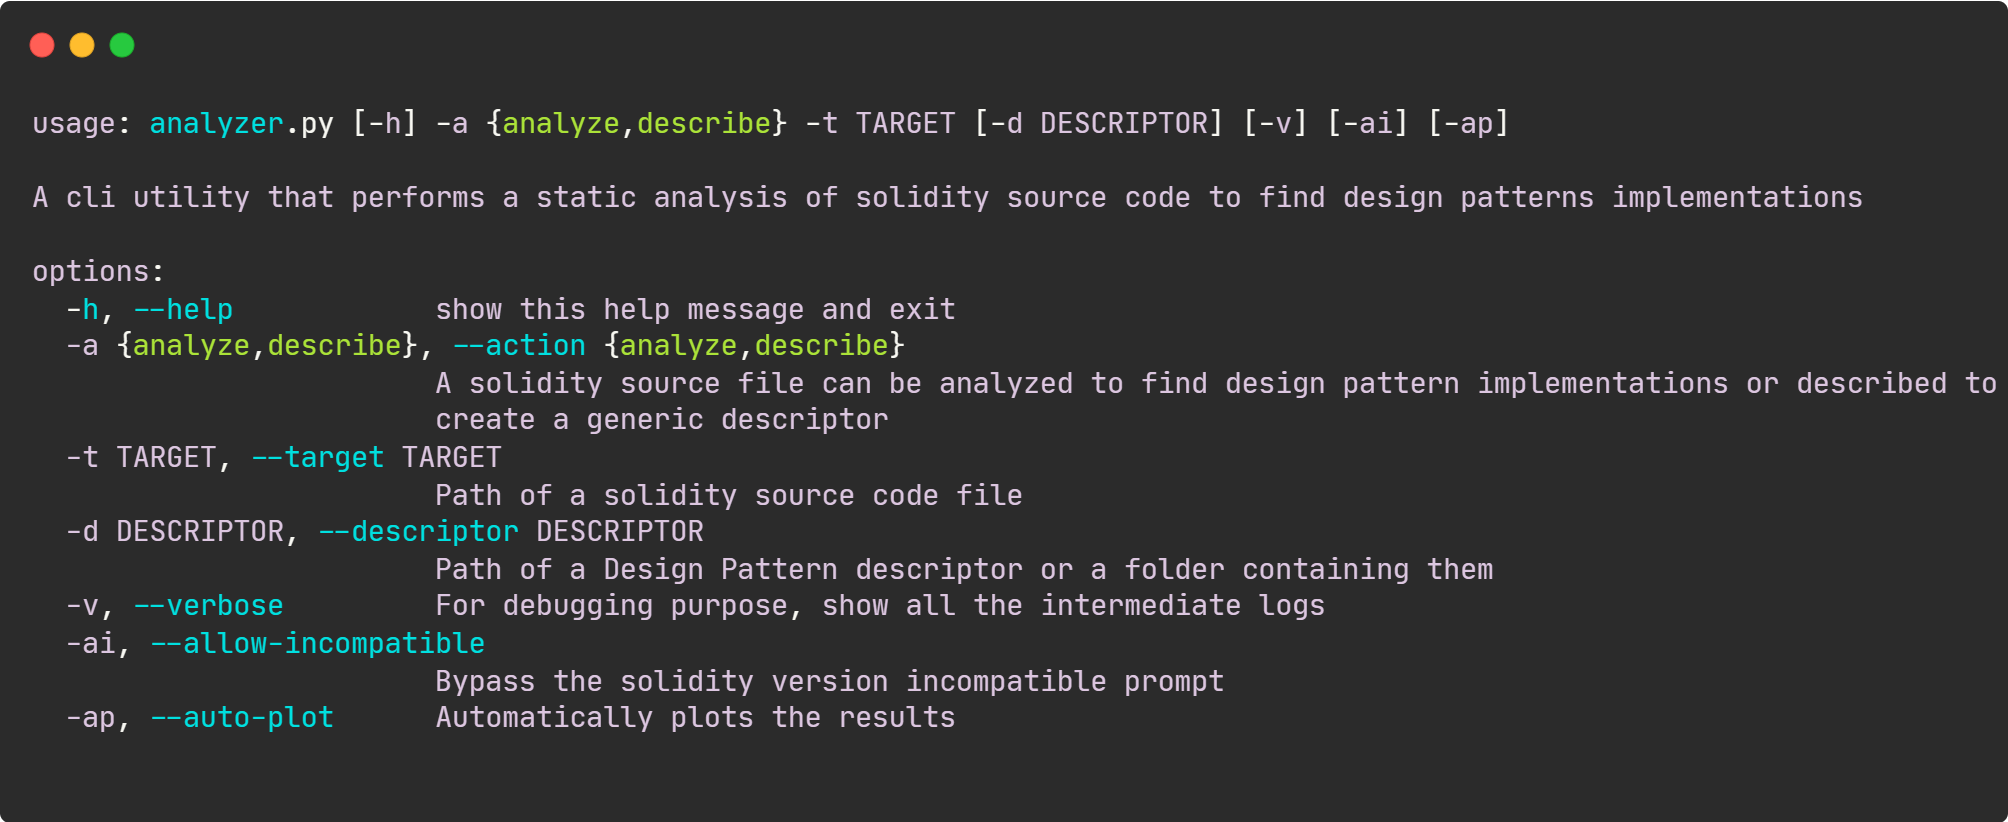
\includegraphics[width=\linewidth]{analyzer-tooltip}
	\caption{Manuale delle istruzioni di Analyzer}
	\label{analyzer-help-tip}
\end{figure}
L'applicativo software sviluppato è denominato \textit{"Solidity Design Pattern Analyzer"}, a cui, per semplicità, sarà fatto riferimento tramite l'abbreviazione \textit{"Analyzer"}.\\
\newline
Analyzer è un programma a riga di comando sviluppato in Python 3, e quindi supportato su MacOS, Linux e Windows, che prende in input il codice sorgente di un contratto, esegue una computazione e restituisce i risultati all'utente.\par
Lo scopo principale di Analyzer è automatizzare il processo di analisi statica del codice sorgente di uno smart-contract con l'obiettivo di individuare quali design pattern siano stati utilizzati.\par
Secondariamente, è possibile utilizzare Analyzer per \textit{descrivere} uno smart-contract, ovvero estrarre, tramite il processo di analisi statica, le informazioni utili a rappresentare un design pattern.

\section{Uso del programma}
Analyzer fa uso di librerie esterne, come ad esempio \textit{python-jsonschema}\cite{JSON-Schema} e \textit{matplotlib}. Per questo motivo, prima di poter utilizzare il programma è necessario installare tramite \textit{"pip"}, il package installer di Python, le dipendenze in uno dei seguenti modi:
\begin{itemize}
	\item \textit{Global Package}: installare le dipendenze direttamente nel sistema, diventando di fatto globali e accessibili da qualunque script Python eseguito nel sistema;
	\item \textit{Virtual Environment}: creare un ambiente virtuale in cui installare le dipendenze;
\end{itemize}
Una volta installate le dipendenze, per utilizzare Analyzer è necessario fornire una serie di parametri, qui elencati:
	\begin{table}[H]
	\centering
	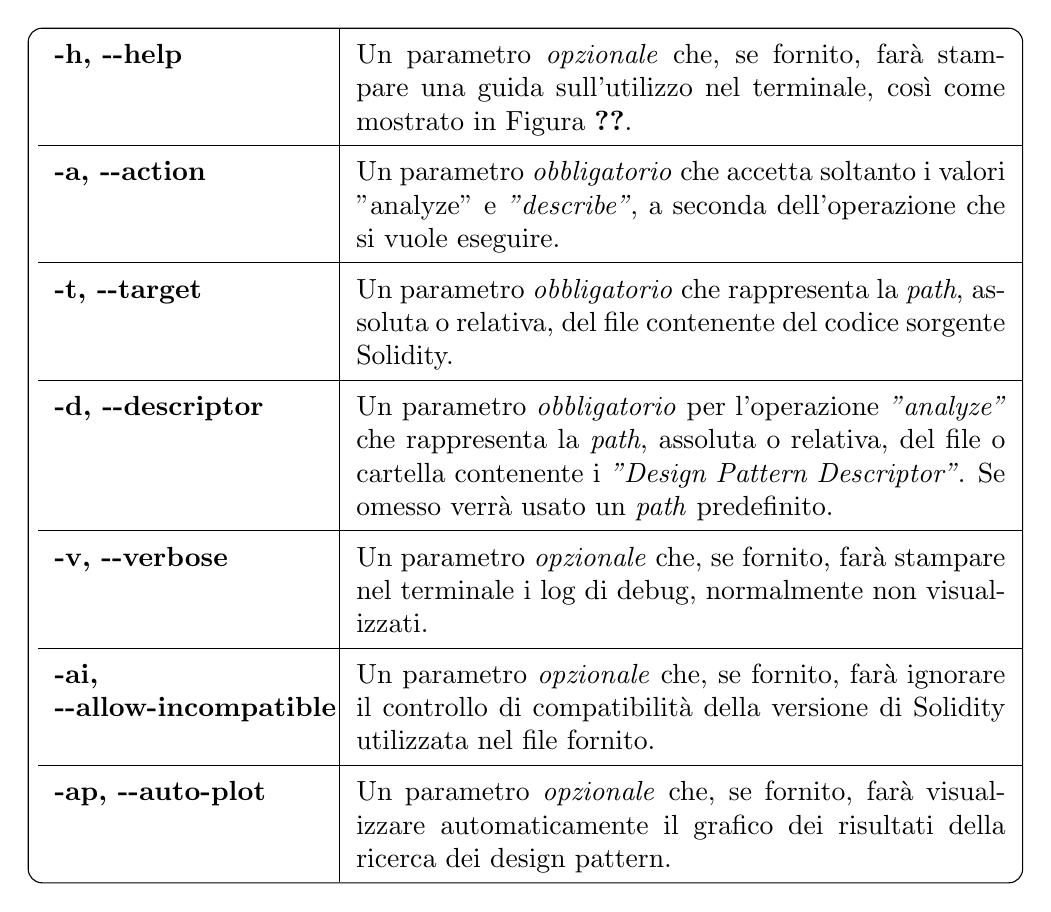
\begin{tikzpicture}
		\node (table) [inner sep=0pt] {
			\def\arraystretch{1.5}
			\begin{tabular}{p{0.28\linewidth} | p{0.68\linewidth}}
				\textbf{-h, -\/-help} & {Un parametro \textit{opzionale} che, se fornito, farà stampare una guida sull'utilizzo nel terminale, così come mostrato in \mbox{Figura} \ref{analyzer-help-tip}.} \\ \hline
				\textbf{-a, -\/-action} & {Un parametro \textit{obbligatorio} che accetta soltanto i valori \textit\mbox{"analyze"} e \textit{"describe"}, a seconda dell'operazione che si vuole eseguire.} \\ \hline
				\textbf{-t, -\/-target} & {Un parametro \textit{obbligatorio} che rappresenta la \textit{path}, assoluta o relativa, del file contenente del codice sorgente Solidity.} \\ \hline
				\textbf{-d, -\/-descriptor} & {Un parametro \textit{obbligatorio} per l'operazione \textit{"analyze"} che rappresenta la \textit{path}, assoluta o relativa, del file o cartella contenente i \textit{"Design Pattern Descriptor"}. Se omesso verrà usato un \textit{path} predefinito.} \\ \hline
				\textbf{-v, -\/-verbose} & {Un parametro \textit{opzionale} che, se fornito, farà stampare nel terminale i log di debug, normalmente non visualizzati.} \\ \hline
				\textbf{-ai, \mbox{-\/-allow-incompatible}} & {Un parametro \textit{opzionale} che, se fornito, farà ignorare il controllo di compatibilità della versione di Solidity utilizzata nel file fornito.} \\ \hline
				\textbf{-ap, -\/-auto-plot} & {Un parametro \textit{opzionale} che, se fornito, farà visualizzare automaticamente il grafico dei risultati della ricerca dei design pattern.} \\
			\end{tabular}
		};
		\draw [rounded corners=.5em] (table.north west) rectangle (table.south east);
	\end{tikzpicture}
	\caption{Descrizione dei parametri di Analyzer}
\end{table}
\noindent Il parametro \textit{"action"} determina che tipo di operazione Analyzer debba eseguire sul file fornito:
\begin{itemize}
	\item \textit{analyze}: effettua la ricerca dell'utilizzo di design pattern e restituisce i risultati in formato JSON, opzionalmente è possibile visualizzare un grafico riassuntivo;
	\item \textit{describe}: estrae le informazioni utili a rappresentare un design pattern e restituisce i risultati in formato JSON, costituendo un \textit{descriptor};
\end{itemize}
Entrambe le operazioni si basano sulla tecnica di analisi statica.\par
Per esempio, volendo analizzare uno smart-contract al fine di individuare l'utilizzo dell'\textit{Ownership} pattern è necessario eseguire il comando:
\begin{lstlisting}[language=bash]
	$ python analyzer.py -a analyze -t ./source_code.sol -d ./Ownership_descriptor.json
\end{lstlisting}

\section{Genericità dell'analisi statica}
Allo scopo di ottenere un sistema flessibile e facilmente estendibile si è deciso di implementare controlli generici  

\section{Design Pattern Descriptor}
Definiti i controlli supportati da Analyzer, è possibile definire un \textit{Design Pattern Descriptor} come un \textit{oggetto JSON} contenente una raccolta di uno o più controlli opportunatamente parametrizzati al fine di individuare uno specifico design pattern.\par
Come esempio, si riporta il descriptor dell'\textit{Auto Deprecation} pattern:
	{\begin{lstlisting}[language=json, caption={Auto Deprecation Descriptor}]
{
	"name": "Auto Deprecation",
	"checks": [
	{
		"check_type": "inheritance",
		"parent_names": ["deprecatable"]
	},
	{
		"check_type": "modifier",
		"modifiers": ["willDeprecate", "whenDeprecated"]
	},
	{
		"check_type": "comparison",
		"binary_operations": [
		{
			"operator": ">",
			"operand_1": "timestamp",
			"operand_2": "expire"
		}]
	}]
}\end{lstlisting}}
\subsection{Affinamento dei parametri dei descriptor}
Per individuare un design pattern, la correttezza dei parametri dei controlli utilizzati è fondamentale. Un parametro troppo generico può causare dei falsi positivi, viceversa può ridurre le probabilità di riconoscimento.\par
Al fine di migliorare i parametri, estratti dai codici di riferimento riportati in \hyperref[appendix:codici]{Appendice}, si è analizzata la libreria \textit{OpenZeppelin Contracts}\cite{openzeppelin}, una libreria per lo sviluppo di smart-contract sicuri, costituita da una solida codebase verificata dalla comunità.\par Data la sua diffusione, si è utilizzato Analyzer per estrarre informazioni utili da utilizzare come ulteriori parametri.



\section{Ricerca di Design Pattern}
Fornendo il valore \textit{"analyze"} come parametro \textit{"action"} viene effettuata la ricerca di design pattern nel codice sorgente fornito in input. L'esecuzione di questa operazione può essere essenzialmente suddivisa in tre fasi:
\begin{itemize}
	\item \textit{Bootstrap}: 
\end{itemize}